% PLEASE FILL IN THE PLACEHOLDERS <...>
%
% Diplomarbeit/Studienarbeit/IDP von <NAME>
% Diploma thesis of <NAME>
%
% Title: <TITLE>
%        <TITLE>
%
\documentclass[12pt, a4paper, twoside, openright]{report}

%%%%%%%%%%%%%%%%%%%%%%%%%%%%%%%%%%%%%%%%%%%%%%%%%%%%%%%%%%%%

% PACKAGES:

% Define typearea
% a) Use automatic:
\usepackage[BCOR1cm]{typearea}
% b) Or use fixed: 
%\usepackage{geometry}
%\geometry{left=1.5cm,textwidth=18.5cm,top=1.5cm,textheight=26.5cm}

% Use German :
\usepackage[german, english]{babel}
% Use list of tabels, etc. in table of contents:
\usepackage{tocbibind}
% German paragraph skip
\usepackage{parskip}
% Encoder:????
%\usepackage[utf-8]{inputenc}
\usepackage[utf8]{inputenc}
% Use A4-paper efficiently:
\usepackage{a4wide}
% Index-generation
\usepackage{makeidx}
% Einbinden von URLs:
\usepackage{url}
% Include .eps-files (needed also for the LKN-logo):
%\usepackage{epsf}
\usepackage{epsfig}
\usepackage{epstopdf}
% Special \LaTex symbols (e.g. \BibTeX):
\usepackage{doc}
% Include Graphic-files:
%\usepackage{graphics}
% Include Graphic-files:
\usepackage{graphicx}
% Include doc++ generated tex-files:
%\usepackage{docxx}
% Include PDF links
%\usepackage[pdftex, bookmarks=true]{hyperref}
\usepackage{float}
\usepackage{tabularx}
\usepackage[margin=1cm,font=small,labelfont=bf,textfont=sl]{caption}
\usepackage{mathtools}
\usepackage[numbers]{natbib}
\usepackage{amssymb}
\usepackage{amsmath}
\usepackage{algorithm}
\usepackage[noend]{algpseudocode}
\usepackage{afterpage}

\usepackage[pdftex,
  bookmarks,
  %colorlinks=false, % instead of colors, now boxes are used for links
  colorlinks=true,
  urlcolor=black, %blue,
  linkcolor=black, %red, %normal internal links
  citecolor=black, %green, %citation links
  %pagebackref, %link from references back to page of citation
  linktocpage, 
  % im Inhaltsverzeichnis Link auf Seitenzahl (sonst Probleme bei langen Zeilen)
  %breaklinks = true, % f�r Links l�nger als 1 Zeile
  %hypertexnames = false,  % f�r Links zu Figures?
  bookmarksopen, %open all bookmark folders
  bookmarksnumbered, %use section numbers with bookmarks
    pdfpagemode=UseOutlines, %show bookmarks
  % http://www.tex.ac.uk/cgi-bin/texfaq2html?label=pdfpagelabels
  plainpages=false, % eigene Seitenanker f�r r�mische/arabische Seitenzahlen
  pdfpagelabels, % im Abode Reader Seitenzahl als z.B. "iii (3 von 20)" anzeigen
% pdfstartview=FitH
  pdfstartview=FitV
  ]{hyperref}

%%%%%%%%%%%%%%%%%%%%%%%%%%%%%%%%%%%%%%%%%%%%%%%%%%%%%%%%%%%%

% SELF DEFINED:
%
% this makes list spacing much better.
%
\newenvironment{my_enumerate}{
\begin{enumerate}
  \setlength{\itemsep}{1pt}}{\end{enumerate}
}
\DeclareMathOperator*{\argmax}{arg\,max}
\newcommand{\sml}[1]{\mbox{\scriptsize $#1$}}

%%%%%%%%%%%%%%%%%%%%%%%%%%%%%%%%%%%%%%%%%%%%%%%%%%%%%%%%%%%%

% OTHER SETTINGS:

% Pagestyle:
\pagestyle{headings}

% Avoid 'overhang':
\sloppy

% Choose language
\newcommand{\setlang}[1]{\selectlanguage{#1}\nonfrenchspacing}

%%%%%%%%%%%%%%%%%%%%%%%%%%%%%%%%%%%%%%%%%%%%%%%%%%%%%%%%%%%%

% TITLE:

\begin{document}

\thispagestyle{empty}
\newpage

\vspace{5cm}
% \begin{center}
%     \epsfxsize=4cm
%     \epsfbox{LKN_Logo_klein.eps}
% \end{center}
\begin{figure}[H]
  \centering
    \includegraphics[width=.6\textwidth]{figures/logo_tuhh.pdf}
\end{figure}

% \parbox{15cm}{\begin{center} {\sf\bf 
%                                \Large  Technische Universität München
%                                 \smallskip

%                                \Large Lehrstuhl für Kommunikationsnetze
%                                \smallskip
%                               }

%                               {\sf \large Prof. Dr.-Ing. Wolfgang Kellerer} 
%               \end{center}}  %&
\begin{center}
\vspace{2cm}

\begin{minipage}{.9\linewidth}
{\centering\Large\bf Indoor Human Tracking based on Dynamic Models from Convolutional Neural Networks \par} 
% \par ist nötig für korrekten Zeilenabstand im Titel
\end{minipage}

\large 

%\vspace{1.5cm}
%{von\\[.3cm] {\bf \LARGE Autor}\\[1cm] 
%\huge  { \bf \it Diplomarbeit} \\[1cm]}

\vspace{1.5cm}
{\large{\bf \it Master Thesis} %\\[1cm]
}

\vspace{0.2cm}
{
\large by \\[.1cm] 
{\bf \large Liangcheng Fu}\\[1.5cm]
}

\vfill
\begin{tabular}{ll}
Start date:& 01 August 2017\\
End date:& 30 January 2018\\
\\
First Examiner:&  Prof. Alexander Schl\"afer\\
Second Examiner:&  Prof. Dr.-Ing. habil. Udo Z\"olzer\\
Supervisor:&  Johannes D\"ollinger\\
\end{tabular}
\end{center}

\vspace{2cm}
\begin{figure}[ht]
\centering%%% not \center
%\subfigure[Figure A]{\label{fig:a}\includegraphics[width=60mm]{example-image-a}}
\includegraphics[width=.35\textwidth]{figures/logo_mtec.pdf}
\hspace{40pt}
\includegraphics[width=.45\textwidth]{figures/bosch_logo.png}
\end{figure}

\afterpage{\thispagestyle{empty}}
\cleardoublepage

%%%%%%%%%%%%%%%%%%%%%%%%%%%%%%%%%%%%%%%%%%%%%%%%%%%%%%%%%%%%
\pagenumbering{roman}

\newcounter{pageno}
\setcounter{pageno}{1} %titlepage = page 1, but pagenumber not printed
\addtocounter{pageno}{1}

% German abstract:
%\include{Kurzfassung}
% English abstract:

%!TEX root = ThesisLKN.tex
\pdfbookmark[1]{Abstract}{sec:abstract}  % Bookmark im pdf file
\chapter*{Abstract}
\label{sec:abstract}

With more and more robots deployed in human populated areas, it becomes very urgent to solve a lot of challenges existing in mobile robot applications. Human tracking is one of these challenges, which is essential for robots to successfully cooperate with humans and fulfill their tasks. Bayesian Occupancy Filter (BOF) is a Bayesian filtering method for object tracking on occupancy grids, which has been successfully used in automotive applications. In this thesis work, we extend the BOF with human motion model to deal with human tracking in indoor environments. For each cell on a gird map, the motion model is represented as a set of probability distributions on the exit direction, conditioned on the entering direction of the current cell. In this way, the motion model is able to capture both place dependency and spatial correlation between cells. A Convolutional Neural Network (CNN) is trained to extract motion model from a static map. By learning from simulated human trajectories, the network is able to generalize motion patterns on maps that never been seen before. We demonstrate our tracking method on both simulated and real human tracking datasets. The results show that our method outperforms its baseline method in both cases. Further applications of our method are also discussed, including predicting future occupancies and frequently occupied areas on a static map.


\afterpage{\thispagestyle{empty}}
\cleardoublepage

\pdfbookmark[1]{Statement}{sec:statement}  % Bookmark im pdf file
\chapter*{Statement}
\label{sec:statement}

\vspace{3cm}
\noindent I assure the single handed composition of this master's thesis only supported by declared resources.\\\\
%M�nchen, DD.MM.YYYY \\\\\\\\\\\\


\vspace*{\fill}

Hamburg, 19. December 2016

\noindent \textit{(John Doe)}
\afterpage{\thispagestyle{empty}}
\cleardoublepage

\pdfbookmark[1]{Foreword}{sec:vorwort}  % Bookmark im pdf file
\chapter*{Foreword}
\label{sec:vorwort}

I would like to use this opportunity to express my gratitude to Northern Institute of Technology Management (NIT). I spent two fabulous years with colleagues, staffs and teachers from NIT. What makes these two years so special and unforgettable is not only the excellent education, but also the international atmosphere and the friendships we developed over time.    

I am also appreciated for the help and guidance I received from Prof. Dr. Corneliue Herstatt, Prof. Dr. Christian L\"uthje and from supervisor Dipl.-Ing. Moritz G\"oldner. I am really grateful for their patience over these four months and their attitudes towards scientific researches inspired me a lot.

Special thanks to all my friends who make my study life more enjoyable. Lastly, I sincerely thank my families. Although they live in the other side of the continent, their continuous supports and cares encourage me to step forward.\\

\vspace{2cm}
Hamburg, 19. December 2016

\afterpage{\thispagestyle{empty}}
\cleardoublepage

% Table of contents:
\thispagestyle{empty}
\tableofcontents  
\afterpage{\thispagestyle{empty}}
\cleardoublepage
%\include{toc}
% % Introduction (Einleitung):
% \include{Introduction}

% % Text Body (Hauptteil)
% % Could have multiple chaper-files, e.g.:
% \include{Background}
% \include{Evaluation}
% %  Conclusions (Zusammenfassung):
% \include{Conclusions}
% \include{Formatting}

\listoffigures
\afterpage{\thispagestyle{empty}}
\cleardoublepage

\listoftables
\afterpage{\thispagestyle{empty}}
\cleardoublepage
\setcounter{page}{1}
\renewcommand{\thepage}{\arabic{page}}

%!TEX root = ThesisLKN.tex
\chapter{Introduction}

In recent years, more and more robots are deployed not only in industrial environments but also human populated areas. In order to fulfill their tasks, it is necessary for robots to interact and even cooperate with people. Therefore, tracking the location of people in those environments has gained enormous attentions in robotics community. Besides, with the increasing popularity of artificial intelligence, robots are also expected to be intelligent enough to predict possible future locations of walking human even when encountered with occlusions or missing of sensor data. Enabled by accurate tracking and prediction of human movements, robots are able to have a better understanding of the environment, which will facilitate interactions between robots and humans.

The very fist requirement for a robot to operate is to model the environment. A simple yet effective way is to use occupancy grid map representation of the environment \citep{elfes1989using}. It decomposes the environment into cells with a predefined resolution, and the state of each cell is a random variable with values of either \textit{occupied} or \textit{not occupied}. This representation has been extensively used in many different kinds of robot tasks like simultaneous localization and mapping (SLAM). The classical grid map representation treats the environment as static, which is not always the case in real scenarios. In other words, the environment can be dynamic since objects can move around in the environment. Object tracking addresses dynamics in environment explicitly, since it tracks and predicts how objects move. If there is more than one object involved at the same time, the tracking problem becomes multiple object tracking (MOT). In human tracking systems, the dynamics in environment refer to changes of humans' location along the time horizon (i.e., trajectories). 

Commonly, a tracking system is implemented as a multiple stage pipeline, which consists of object detection, data association, motion modeling and occupancy generation. When dealing with a multiple object tracking problem, data association becomes very tricky. The classical way to perform data association is to maintain a list of known objects, and associates new observations with those existing objects. The main difficulty of this approach is to deal with \textit{birth} (whether observation is from a new object) and \textit{death} (whether a maintained object should be deleted) of tracks \citep{gauvrit1997formulation}. 

To address the data association problem, \citet{coue2006bayesian} proposed \textit{Bayesian occupancy filter} (BOF), which is an object tracking algorithm based on grid map representation of the environment. It essentially avoids data association step in the tracking pipeline, since concepts of \textit{objects} and \textit{tracks} does not exist in BOF framework. Rather than treat tracking problem from an \textit{object} point of view, BOF addresses tracking from a \textit{cell} perspective. That is to say, tracks are replaced by transitions of occupancies between cells over time. Meanwhile, BOF is robust to object occlusion thanks to the combination of \textit{prediction} and \textit{estimation} steps. This two-step mechanism is well suited for handling the consistency between occupancy predictions and new observations, therefore uncertainties incurred by occlusion are naturally handled in a probabilistic way. Over the past few years, there has been some extensions over BOF proposed in literature \citep{gindele2009bayesian, brechtel2010recursive, llamazares2013dynamic}. 

\begin{figure}[H]
  \centering
    \includegraphics[width=.5\textwidth]{figures/roundabout.png}
    \caption[An illustration of a round-about]{Illustration of a round-about. Cars can only drive in directions indicated by red arrows. The green rectangle represents a car at that location. Since we know that the car must drive in the specified directions, the possible locations of the car after a few time steps are indicated by the two green ellipses. This prior knowledge helps us to track the dynamic objects since we have better chances to locate the car according to its motion pattern.}
    \label{fig:roundabout_idea}
\end{figure}

A tracking system usually predicts the state of the world (e.g., object location and velocity) based on past observations. Many tracking algorithms also incorporate motion model of the objects being tracked, since this allows them to utilize prior knowledge of object's motion cues. As an intuitive example, let us consider a round-about as shown in Figure \ref{fig:roundabout_idea}, where cars can only drive in one direction. To track a car driving in a round-about, predictions of future possible locations of the car should always be on the side which allowed driving direction indicates. Likewise, human tracking in indoor environments can also benefit from human motion patterns. For BOF and its variants, the objects being tracked are assumed to perform linear motion, which indicates that objects always move in the same direction as in the last time step. Although \citet{gindele2009bayesian} proposed to incorporate prior map knowledge (BOFUM) to better model the motion dynamics based on cell context, the underlying linear motion is too simplistic to model actual human motion in indoor environments. 

Based on our observations of human trajectories, we found two aspects very important for explaining human motion: 1) Unlike in free space, people have to move under spatial constraints in indoor environments. For example, people tend to walk along the central area between walls in a corridor and change their walking directions when they have to make turns. That is to say, the spatial configuration puts constraints on human motion patterns and therefore human motion is very place dependent. 2) People move continuously in time and space, which means they do not disappear or appear out of thin air. If a person is currently located at a cell on a grid map, he or she has to walk through its neighboring cells first. In other words, future state of a cell is highly influenced by state changes of its neighboring cells. These observations motivates us to model human motion in a way that captures both \textbf{place dependency} as well as \textbf{spatial correlation} between cells.

In computer vision community, machine learning has shown a lot of successes over last few years . Image classification algorithms based on convolutional neural networks (CNNs) won all ImageNet classification challenges since 2012 \citep{russakovsky2015imagenet}. It turns out that CNNs achieve good results in not only computer vision tasks but also many other domains. For example, recurrent neural networks (RNNs) can be applied in automatic language translation \citep{cho2014learning}. Deep reinforcement learning are good choice for teaching robots to perform human actions like grasping\citep{levine2016learning}. Essentially, the reason why CNN works in those domains is that it is able to capture complex structures in data. Once a CNN learns these structures, it can generalize to cases that never occur during training. 

In order to utilize the powerful generalization abilities of CNNs, we proposed to model motion patterns in a way that can be expressed as the output of a CNN. By this way, if we feed a grid map as input and human motion pattern as ground truth to a network, it is able to learn the pattern after training with lots of data. We model human motion patterns as a set of conditional probabilities for every cell on the map. They represent how likely a person moves to one of the neighboring cells, conditioned on which neighboring cell he or she comes from. Since these probabilities incorporate information about the incoming cell, the motion model captures spatial correlations between cells. Besides, they are different for each cell based on cell's context on the map, which means that the learned motion pattern is expressive enough to predict different motions at different locations. In other words, our motion model is also place dependent. In fact, similar idea of making motion patterns place dependent has been proposed by \cite{kucner2013conditional}, but in order to learn motion pattern on a map, they need sensor observations from that specific map. In other words, their method lacks generalization ability. 

\begin{figure}[H]
  \centering
    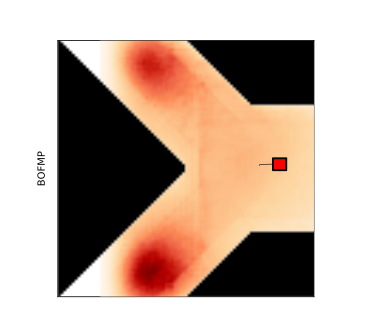
\includegraphics[width=.6\textwidth]{figures/theme_plot_1.png}
    \caption[An example of future occupancy predictions of our method.]{An example of future occupancy predictions of our method.  The map shows a Y-fork, where only white spaces are walkable. Initially, a person is shown as a red rectangle and with velocity towards left. Since no further sensor reading is given, BOFMP propagates occupancies over time. After some time interval, most occupancies appear in both upper and lower branches of the corridor, which proves that our motion model successfully learns that people tend to make turns at the intersection. Besides, BOFMP predicts more occupancies in the middle of corridors, since it learned that people are less likely to walk near walls.}
    \label{fig:intro_idea}
\end{figure}

The data we use for training network is generated from simulated human trajectories on SLAM-generated maps of real world offices. Once the network finishes learning, we can feed new maps to the network and obtain human motion patterns from network output. These motion patterns are then incorporated into the BOF framework to perform human tracking in indoor environments. We call our tracking method \textit{Bayesian Occupancy Filter with Motion Patterns} (BOFMP). If only initial state of a person is given and no further observations are provided, our method is able to predict reachable areas after some time steps. Figure \ref{fig:intro_idea} shows an example of future occupancy predictions of our method without sensor observations. It shows that our way of modeling human motion patterns enables BOF to propagate occupancies to reasonable areas.

The main contributions of this thesis are:

\begin{my_enumerate}
\item We present a way of modeling human motion patterns that captures both place dependency and spatial correlations between cells. Besides, thanks to powerful generalization abilities of CNNs, our method can generate motion patterns on maps that are never seen by our network.
\item We incorporate the learned motion patterns into BOF framework seamlessly for human tracking in indoor environments, and achieve better tracking performance than the baseline method.  The whole pipeline of modeling motion patterns and tracking of dynamic objects presented in this thesis work can be applied in other scenarios, such as car tracking in ADAS systems.
\end{my_enumerate}


The rest of this thesis is organized as follows: Chapter \ref{chapter:2} summarizes the related works and highlights the similarities and differences between our method and others in literature. Chapter \ref{chapter:3} introduces mathematical formulation of BOFMP and discusses how the network structure used in thesis is derived. Chapter \ref{chapter:4} talks about some details on the implementations, such as simulation of human walking trajectories and the code structure of BOFMP. Chapter \ref{chapter:5} summarizes the dataset and presents the tracking performance of our method and its baseline. Chapter \ref{chapter:6} concludes the thesis and presents possible improvements on our method. 


\cleardoublepage
%!TEX root = ThesisLKN.tex
\chapter{Literature Review} \label{chapter:2}

This chapter lists literatures that are related to methods or concepts used in this thesis work. Section \ref{lr:tracking} discusses two classical ways of tracking object and introduces BOF and its variants. Section \ref{lr:dynamic} presents literatures that try to model dynamics in environment. Section \ref{lr:network} details recent researches on neural networks and relations between RNNs and Bayesian filters. 

\section{Object Tracking} \label{lr:tracking}

Perception of environment can be done with different sensors, which also differentiates object tracking applications. Visual tracking refers to object tracking with RGB cameras \citep{ross2008incremental}. In this thesis work, however, we mainly concern object tracking with 2D laser scanners. 

One popular paradigm of performing tracking is tracking by detection: moving objects are firstly detected and then determine how to pair them with existing tracks. Generally, there are two approaches to deal with detection based object tracking: \textit{model-free} and \textit{model-based} \citep{wang2015model}. The detection of model-free object tracking works based on motion cues. In this case, prior knowledge on neither object's semantic information (whether it is a car or a person) nor object's shape or geometric properties is needed. However, this approach only tracks objects that show instantaneous motion dynamics and potential moving objects might be neglected. BOF can be regraded as a model-free tracking algorithm (but not within tracking by detection paradigm) since it predicts occupancies based on its inference on cells' velocities. Similar to BOF, \citet{ross2008incremental} models the environment with occupancy gird map. Their work combines SLAM with dynamic object tracking in outdoor environment. Once the vehicle equipped with laser sensors is self-located and objects are detected by motion cues, they apply a method called Global Nearest Neighborhood (GNN) for tracking. On the contrary, for model-based tracking, semantic class of the objects being tracked is given, and detection is done with the help of a parametric model of the object's shape. For human tracking, a person is normally represented as point blob or modeled based on detection of legs \citep{arras2008efficient, cui2006laser}. 

The tracking by detection paradigm has to address \textit{data association} explicitly, which is known to be as the main difficulty in tracking. Data associations refers to match detections of moving objects in new observations to a set of tracked trajectories from last time step. To address data association problems in tracking, many methods have been proposed in literature. Historically, nearest neighbors based approaches are used in the early stage \citep{fod2002laser}. \citet{schulz2001tracking} detect people by their legs in 2D laser scans and propose the Joint Probabilistic Data Association Filter (JPDAF) for tracking. \citet{arras2008efficient} is similar in identifying people with legs but their tracking is done with Multi-hypothesis tracking (MHT). Although the mentioned methods partially address the data association problem, their performance is not stable in densely cluttered environments, where occlusions happen quite often.

On the contrary to tracking by detection paradigm, tracking can also be done without detection, e.g., tracking by filtering. \citet{coue2006bayesian} propose Bayesian Occupancy Filter for object tracking in automotive applications. The environment is represented by a grid map, and the state of each cell is characterized by its occupancy and velocity. Inspired by Bayesian Filter, tracking works in a form of recursive \textit{predictions} and \textit{estimations} of cells' state. One of important advantages of BOF is that the concepts of \textit{objects} and \textit{tracks} are replaced by transitions of occupancies between cells over time. That is to say, data association is addressed implicitly by BOF. Later works extend BOF to better adapt to real world situations. BOF's linear motion model cannot adapt to traffic scenarios like curved roads. Therefore, \citet{gindele2009bayesian} propose to enrich motion model of BOF with prior map knowledge (BOFUM), which can be obtained from navigation systems. By this way, BOFUM predicts occupancies according to motion preferences at different locations, which results in reliable estimates even when occlusion happens. 

Despite of various variants of BOF, all of them assume that objects perform linear motion. However, linear motion is obviously over-simplified for real world scenarios. Besides, since objects cannot appear or disappear suddenly, the state changes of a cell's neighboring cells contain valuable information for prediction of its future state. Therefore, we proposed to model human motion patterns in a way that captures both place dependency and spatial correlation of cells. This motion model is then incorporated into BOF framework to perform human tracking. A similar idea is used in the work of \citet{luber2011place}, which proposed a place dependent people tracking algorithm. Unlike BOF which tracks objects by filtering, they perform people tracking by detection and data association. They proposed to model human activity events as a three-layer spatial affordance map with each layer characterizing the probability distribution of new tracks, matched tracks and false alarms respectively. Each layer is represented by a \textit{spatial} Poisson process which introduces spatial dependency and the parameter of each cell is learned from a sequence of observations. Figure \ref{fig:affordance} shows one example of two layers of the learned spatial affordance map. Their motion model is place dependent because the parameters of Poisson processes are different on the spatial affordance map. They use boosted features for people detection \citep{arras2007using} and they extend multiple hypothesis tracking (MHT) for data association. Their results show they achieve more accurate tracking behavior in terms of data association errors. 

\begin{figure}[H]
  \centering
    \includegraphics[width=\textwidth]{figures/affordance_map.png}
    \caption[Two layers of a spatial affordance map.]{Two layers of a learned spatial affordance map \citep{luber2011place}. On the left shows probability distribution of matched track events, and on the right shows that of new track events. Note that the maxima appear in different regions in two maps. While on the left the maxima appear at places frequently used by people (e.g., desks and coach), on the right the maxima of new track events indicate places where people normally appear from, i.e., doors.}
    \label{fig:affordance}
\end{figure}

\section{Dynamics Modeling} \label{lr:dynamic}

Nowadays, more and more robots are entering dynamic environments. In order to fulfill their task, it is imperative for robots to understand these dynamics. In the context of human tracking, these dynamics refer to human movements in the environment. In literature, some researchers try to model human dynamics \textit{explicitly} by a motion model. Meanwhile, others model them \textit{implicitly} by regarding human dynamics as part of the environment and therefore model the environment directly. We discuss dynamics modeling according to these two approaches. In both cases, we represent the environment as a gird map with each cell representing a possible location. 

\subsection{Human Motion Modeling}

In the early stage of human tracking, researches adopts simple and conservative motion models. \citet{montemerlo2002conditional} uses Brownian motion model for human tracking with Bayesian filters.  The Brownian motion assumes people take random directions at each time step and there is no dependence between time steps. In other words, Brownian motion does not assign human dynamics with any pattern other than dispersion. As a consequence, when there is no observations, predictions of people locations spread out over a large area very quickly. This is a poor estimate as we know people does not move randomly. In reality, people normally go from the starting point and follow some motion patterns until they reach destination. A more realistic model is the first order motion model (a.k.a. linear motion model). For example, \citet{meier1999using} used this model together with Kalman filter for human tracking. First order motion model assumes people always move in the same direction as in the last time step. This assumption might be true if a person is walking along a straight corridor, but in many cases it is invalid because people often need to make turns around corners. Some researchers proposed better ways to model human motion patterns. For example, \citet{bruce2004better} propose to learn destinations by clustering real trajectories and use a path planer to those destinations as a reference for human motion patterns. \citet{liao2003voronoi} observe that human tend to move along Voronoi graph of the environment and therefore constraint motion patterns by Voronoi graph. 

Our motion model is different to above methods in two aspects: fineness and cell dependency. The Voronoi graph is constructed based on a \textit{global} representation of the environment. It is predefined and only well suited for applications where high-level motion clue is needed (e.g., which rooms a person has visited). This kind of motion clues are too less precise to be used for recovering a person's exact location. Therefore, in order to get a finer motion model, we decompose the \textit{global} task of modeling human motion pattern into \textit{local} tasks at cell level. On the other hand, although a path planer to the learned destination defines an effective path, it does not necessarily cover the motion dynamics at every possible locations and it also assumes no dependency between these locations. One intuition we captured based on observations of human motion is that, for a cell in the map, the state changes of its neighboring cells is a strong indicator for predictions of its future state. To capture this \textit{spatial} correlation, we propose to model changes of movement directions. For each cell, we learn from human trajectories how likely a person's moving direction changes for the next time step, conditioned on the direction with which he or she enters this cell. Moreover, this way of motion modeling also captures \textit{temporal} correlations, since it builds connections for each cell with its neighboring cells from both last time step and next time step. 

In fact, after we came up with above way of modeling human motion, we found in literature the same idea has been used by \citet{kucner2013conditional} in an autonomous navigation scenario. Their model, which is named as Conditional Transition Map, is created by ``learning the probability distribution of an object leaving to a certain neighboring cell, given the cell from which it entered into the current cell.'' They demonstrate their method with a roundabout, and the corresponding model is illustrated in Figure \ref{fig:condi_tran_map}. One can see that at different locations in the roundabout, different motions are learned, which accurately models how cars drive through the roundabout. The difference between our method and theirs lies in how those probabilities are learned. The cross-correlation of temporal occupancy signals extracted from observations is used for learning in their method, while our model learns these probabilities by training a neural network. With lots of different maps as training data, our network is able to learn the motion patterns that are constrained by spatial configurations of these maps. One of the most important advantages of our method is that our network can generalize motion patterns for maps that never occur in training data. Therefore, our method can work in new environments without learning these probabilities from scratch. 

\begin{figure}[H]
  \centering
    \includegraphics[width=.6\textwidth]{figures/condi_tran_map.png}
    \caption[Conditional transition map of a roundabout.]{Conditional transition map of a roundabout \citep{kucner2013conditional}. Arrows indicate the exit directions for that cell. For simplicity, the entering directions are not drawn. One can see that this model captures how cars drive through the roundabout. }
    \label{fig:condi_tran_map}
\end{figure} 

\subsection{Dynamic Environment Modeling}

For a mobile robot to operate, a proper way to model the environment is necessary. \citet{elfes1989using} introduces occupancy grid as a representation of environment, which divides the environment into a grid of cells with a predefined resolution. Each cell is a random variable with values of either \textit{occupied} or \textit{not occupied}. The occupancy grid assumes the environment being static, which does not hold in real world situations. For example, a robot might need to work in a traffic intense environment with driving cars and pedestrian. 

Early attempts to model dynamics in environment extend occupancy gird with a timescale framework. \citet{arbuckle2002temporal} propose to model dynamics with a stack of occupancy grids with each layer corresponding to a different timescale. They call this representation Temporal Occupancy Grid (TOG). Objects' motion pattern can then be classified based on their occupancy traces across different layers of TOG. For example, if a cell is occupied across all layers of TOG (i.e., occupied at all timescales), it is likely to be a part of the background. Similarly, traffic patterns with various speeds can be identified based on their occupancy traces on a certain layer of TOG. \citet{biber2009experimental} use multiple map representations of the dynamic environment with different timescales for long-term SLAM. Mapping is refreshed based on a sample set of observations that is updated over time by random replacement. Different timescales relates to different learning rate. Map with higher learning rate adapts to new observations faster than these with lower learning rates.

Although the above methods can be applied for modeling dynamics, essentially their static nature remains if we look at each layer that characterizes a specific timescale. In order to capture the dynamic nature of environment, \citet{meyer2012occupancy} propose to model state changes of cells by a two-state hidden Markov models (HMMs). Therefore, the dynamics in environments are explicitly characterized by the state transition probabilities of HMMs. The parameters of these HMMs are estimated with an Expectation Maximization (EM) algorithm. 

However, although their method relaxes the static cell state assumption made by occupancy grid, they assume that state changes of cells are caused by a \textit{stationary} process. In other words, a cell's state transition probabilities are constants over time. Moreover, the assumption of independences between cells is not always valid since state change of a cell's neighboring cells is a strong indicator of that cell's future state. Due to above reasons, cell-specific input-output HMMs (IOHMMs) are used by \citet{wang2014modeling} to better model dynamic environments. An IOHMM imposes conditional dependences on latent variable and observed variable with an input sequence. An illustration of IOHMM used in their method is depicted in Figure \ref{fig:IOHMM}. The input sequence is determined by past observations of neighboring cells. By this way, the transition model of their method is adaptive to input sequence that varies over time, which relaxes the assumption of stationary process made by \citet{meyer2012occupancy}. It also incorporates spatial correlations by making input sequence dependent on neighboring cells. 

\begin{figure}[H]
  \centering
    \includegraphics[width=.6\textwidth]{figures/IOHMM.png}
    \caption[An illustration of IOHMM.]{An illustration of IOHMM used by \citet{wang2014modeling}. Note in this IOHMM only latent variables are dependent on input sequence, which is determined by past observations in neighboring cells.}
    \label{fig:IOHMM}
\end{figure} 

Our method is conceptually equivalent to theirs. In both methods, the influence of neighboring cells is captured by conditional dependence. Although our motion model is fixed for a specific map, the occupancies propagate to a certain cell only when its neighboring cells have velocities towards it. This mechanism acts as a ``trigger'' which only get triggered at certain time and essentially makes our model time dependent.


\section{Neural Networks} \label{lr:network}

Since \citet{krizhevsky2012imagenet} applied deep convolutional neural networks (CNNs) in large scale image classification in 2012, CNNs have gained a lot of successes in computer vision. Researches show that the depth of network plays a very important role in CNNs' performance \citep{simonyan2014very}. However, deep networks are more difficult to train, possibly due to poor gradient flow during back-propagation. To address this problem, \citet{he2016deep} propose to fit a \textit{residual} mapping with stacked layers of CNNs instead of fitting the desired underlying mapping directly. This idea is implemented as ``shortcut connections'' between layers. A shortcut connection branches from one layer and connects to one of the followed layers. Moreover, \citet{huang2016densely} extends the idea of residual learning so that each layer has a shortcut connection to every other layer in the network. This design guarantees layers with easy access to its preceding layers and makes feature reuse very easy. Figure \ref{fig:dense_net} shows a five layer densely connected CNN (DenseNet).  Compared with other CNN structures like ResNets, DenseNets are better at alleviating vanishing-gradient problem and therefore improve classification accuracy with even fewer parameters. 

\begin{figure}[H]
  \centering
    \includegraphics[width=.6\textwidth]{figures/denseNet.png}
    \caption[A five layer dense block.]{A five layer dense block \citet{huang2016densely}. As can be seen, each layer has a shortcut connection to every other follower layer in the network.}
    \label{fig:dense_net}
\end{figure} 

Besides image classification, CNNs have been extensively used in other computer vision tasks like semantic segmentation. Unlike in image classification where only one class has to be determined for the whole image, semantic segmentation requires  classification at pixel level. \textit{Fully} convolutional neural networks have been proposed by \cite{long2015fully} to tackle this problem. By removing fully connected layers and adding a deconvolution layer that functions as upsampling, their network is able to take arbitrary size image as input and predicts pixel-wise classification. Their network also includes skip connections that combine deep coarse features (e.g., semantic information) and shallow fine features (e.g., geometric shape and appearance), both of which are proved to be essential for semantic segmentation. \citet{jegou2017one} extends fully convolutional networks with dense blocks, i.e., a block of convolutional layers that \textit{densely} connected as in DenseNet. Their proposed structure is designed for semantic segmentation, with a downsampling path extracting high-level semantic feature and an upsampling path recovering outputs to full resolution as input image. 

The network structure used in this thesis is similar to that of \citet{jegou2017one}. Since our proposed motion model needs to be place dependent, our network is required to predict probabilities at cell level, which is similar to pixel level prediction in semantic segmentation. The differences lie in the meaning of these probability outputs. For semantic segmentation, these are probabilities of a pixel belonging to a specific semantic class, while in our case they are probabilities of object's exit direction conditioned on which direction it takes to reach current cell.   

As CNNs are good fit for image based tasks, recurrent neural networks (RNNs) are found to be very useful to deal with sequential data such as videos and texts. RNNs have been successfully applied in applications like object tracking \citep{ondruska2016deep}, automatic language translation \citep{cho2014learning} and speech recognition\citep{graves2013speech}. Long short-term memory (LTSM) \citep{hochreiter1997long} addresses vanishing and exploding gradient problems and becomes one of most popular variants of RNNs. 

\begin{figure}[ht]
  \centering
    \includegraphics[width=.7\textwidth]{figures/rnn_and_bayes.png}
    \caption[Comparison between RNN and Bayesian filters.]{Comparison between RNN and Bayesian filters \citep{de2017dynamic}. For Bayesian filers, the dynamics are modeled by a Markov process (red dash lines). In both cases, measurements are fed into the systems as inputs.}
    \label{fig:rnn_and_bayes}
\end{figure} 

\citet{ondruska2016deep} propose a framework named \textit{deep tracking} for object tracking with 2D laser data. Deep tracking uses RNNs as the underlying model, and it is designed to be trained in an end-to-end fashion from raw sensor data without hand-crafted feature engineering. Unlike in most supervised learning applications where human annotated ground truth is needed, they train the network with future sensor observations (i.e., future inputs to network) as ground truth, which essentially makes the training unsupervised. Further, \citet{ondruska2016end} extends their deep tracking framework so that it can perform object tracking and semantic segmentation at the same time. 

The fact that object tracking can be achieved by both Bayesian filter based approaches like BOF and RNN based approaches like deep tracking leads us to understand their connections. In a paper that aims at dynamic facial analysis, \citet{de2017dynamic} try to compare Bayesian filters with RNNs as depicted in Figure \ref{fig:rnn_and_bayes}. Given noisy measurement as input, the goal of Bayesian filter is to estimate the hidden state and optionally the target output, while RNNs sequentially predict target output as a function of hidden state which is in turn dependent on new measurements. The performance of Bayesian filters is highly dependent on how much the assumed transition model and measurement model are close to real situations. While for RNNs, this step of handcrafted engineering is avoided since RNNs are able to model them implicitly by learning from data, which is similar to how CNNs extract features from images without artificial feature engineering. On the other hand, despite its successes in many applications, how the hidden states involve over time and how to interpret the hidden states remain a challenge in understanding RNNs. For Bayesian filter, interpretations of the transition processes are usually quite straightforward. 



\cleardoublepage
%!TEX root = ThesisLKN.tex
\chapter{Background Knowledge} \label{chapter:3}
%
\section{Bayesian Occupancy Filter (BOF)} 

\subsection{Bayesian Filtering}

\subsection{Bayesian Occupancy Filter Formulation}

\subsection{BOF with Map Knowledge and Motion Model}

\section{Fully Convolutional Neural Network}

\subsection{Densely Connected Convolutional Networks (DenseNets)}

\subsection{Fully Convolutional DenseNets}

\section{Metrics}

\cleardoublepage
%!TEX root = ThesisLKN.tex
\chapter{Implementation Details} \label{chapter:4}

\section{Human Trajectory Simulation}

\section{Architecture of Neural Network}

\section{Implementation of BOFUM}

Before tracking starts, the occpancy and velocity probabilities are initialized uniformly, i.e.,

\[ P_c\{ O = occ \}=P_c\{O = nocc\}=0.5  P_c\{V= v \}=1/number \ of \ velocities \] 

\section{Hyperparameter Tuning}



\cleardoublepage
%!TEX root = ThesisLKN.tex
\chapter{Results and Discussions} \label{chapter:5}


\section{Metrics} \label{sec:metrics}

\subsection{Metrics for Neural Network}

\subsection{Metrics for Tracking}

The possible metrics that could be used for measuring the consistency between occupancy predicition and ground truth are: \textit{cross entropy}, \textit{f1 score} and \textit{average precision}.  We choose average precision as our metric and the reasons will be detailed in the thesis.

\section{Training of Neural Network}

After the data is collected as described in Section \ref{sec:traj_sim}, we split them into training, validation and test set. The training and validation set are sampled from seven full maps, and test set is sampled from a separate map. The number of samples we generated are summarized in Table \ref{table:nos}. 

Figure \ref{fig:trajs} shows one example of map window as network input and its ground truth. On the left, a cell is labeled with red color, and the sampled trajectories that go through this cell are displayed. On the right, it shows a visualization of the ground truth \( P_c(V^{ex} | V^{en}) \) for that red cell. The axes show velocities on \( x, y\) directions. Since we assume a person has maximum speed of 1 $cell/timestep$, the velocities must be in range $[-1,1]. $Outer axes represent entering direction \( V^{en} \), and inner represents exit velocity \( V^{ex} \). One can see that \( P(V^{ex}=DL | V^{en}=DL) = 0.13 \) and \( P(V^{ex}=D | V^{en}=DL) = 0.87 \) \footnote{DL represents going down-left, and its corresponding velocity is (-1, -1). D represents going down, and its velocity is (0, -1).}. This indicates that if a person reaches the red cell by taking direction down-left (i.e., coming from upper-right neighboring cell), it is very likely that he or she will change to going down for the next time step. This proves that our way of modeling motion pattern captures human motion dynamics.

\begin{table}[t]
\centering
  \begin{tabular}{c|ccc}
    \hline
     & training & validation & test \\ \hline
    number of samples & 27,119 & 4,785 & 3,760\\
    \hline
  \end{tabular}
\caption{Number of samples in training, validation and test set.}
\label{table:nos}
\end{table}

\begin{figure}[H]
\begin{tabular}{ll}
\includegraphics[width=0.48\textwidth]{figures/trajs_through_cell.png}
&
\includegraphics[width=0.48\textwidth]{figures/probs_on_that_cell_2.png}
\end{tabular}
\caption[one example of map window as network input and its ground truth]{one example of map window as network input and its ground truth \textbf{Left}: The map window has size of \( 32 \times 32 \) cells, with resolution of \( 0.2m/cell\). It also shows trajectories that goes through the red cell. \textbf{Right}: Visualization of conditional probability \( P_c(V^{ex} | V^{en}) \) for the red cell on left map. It can be seen that if a person reaches that cell by taking down-left direction, it is very like that he or she will change direction to going down.}. 
\label{fig:trajs}
\end{figure}

\begin{figure}[ht]
  \centering
    \includegraphics[width=.7\textwidth]{figures/training_hist.png}
    \caption{Cross entropy loss during training. The networks are trained to learn conditional probabilities \( P_c(V^{ex} | V^{en}) \). The blue line shows training dynamics using data generated with 4 directions "left, right, up and down". The yellow line also takes diagonal directions into account, which has 8 directions in total. }
    \label{fig:trainning}
\end{figure}

Practically, the hyperparameters of a neural network, such as learning rate and weight decay, are optimized by random search. However, due to time limitation, this step is skipped in this thesis work. Instead, we use the hyperparamters from a similar network (the only difference is the output layer) that is optimized for predicting average human occupancy on static map. The network is trained with mini-batches of size of 128, and  is optimized with Adam optimizer \citep{Kingma2014Adam}. The training runs for 100 epochs, with early stopping patience of 15 epochs. The best model is selected based on the KL-divergence on validation data.

 Figure \ref{fig:trainning} shows the cross entropy loss during training. We trained networks for two cases: 4 directions and 8 directions. The 4-direction case considers only "left, right, up and down". Therefore, the dimension of its output is $32 \times 32 \times 16$. The 8-direction case considers also diagonal directions, therefore the output dimension is $32 \times 32 \times 64$. The loss curves show that the hyperparameters are set correctly since the loss decreases exponentially in the early stage and keeps decreasing afterwards. Naturally, more directions implies higher complexity, thus the overall loss for yellow line is higher than blue line. The cross entropy on the test set is listed in Table \ref{table:loss_on_test}.

 \begin{table}[H]
\centering
  \begin{tabular}{c|c}
    \hline
     networks      &      cross entropy  \\ \hline
     4-direction   &      0.334 \\ \hline
     8-direction   &      0.383 \\          
   \hline
 \end{tabular}
\caption{Cross entropy loss on test data.}
\label{table:loss_on_test}
\end{table}

\section{Evaluation of Tracking Performance}

Our method BOFMP is proposed for human tracking in indoor environment. It is similar to BOFUM, and we claim it improves BOFUM since it is able to predict occupancy according to human motion pattern. To verify our claim, we compare the performance of BOFUM and BOFMP in two scenarios:

\begin{my_enumerate}
\item \textbf{tracking stage}. Before a certain time point \( t_{lost} \), measurements are given at each time step, i.e., $t=1:t_{lost}-1$. We evaluate consistency between occupancy prediction and the ground truth at every time step.
\item \textbf{future prediction stage}. From time point \( t_{lost} \) on, the measurement is no longer given. Then we evaluate occupancy predictions with ground truth for the next \( n \) time steps.
\end{my_enumerate}

These two stages can be illustrated as:
\[\text{start} \rightarrow \text{tracking stage} \xrightarrow{\text{measurement lost}} \text{future prediction stage} \rightarrow \text{end}\]
In this thesis, we set $t_{lost}=9$ and $n=8$, i.e., both tracking and future prediction stage lasts for 8 time steps. The parameters of filters are tuned based on their performance in \textit{future predictions} stage. 

  % The measurement is lost at time step \( t=9\), and we select the best set of parameters based on the average of average precisions for the next \( 8 \) time steps. 

\subsection{Overview of Datasets}

\textbf{Simulated Dataset}

We generated 500 scenes as training set for tuning filter parameters and 500 scenes for test set. Training and test data are generated from different maps. In these scenes, there are either one or two walking humans. Two examples of scenes in training set are shown in Figure \ref{fig:sample_scene_simulated}.

\begin{figure}[hp]
  \centering
  \includegraphics[width=.99\textwidth]{figures/simulated_dataset_1_persons_with_traj.png}
    \includegraphics[width=\textwidth]{figures/simulated_dataset_2_persons_with_traj.png}
    \caption[Two examples of scenes in simulated training set.]{Two examples of scenes in simulated training set. Each person is indicated by a red square and the lines show the trajectory for each person. \textbf{Up}: This example shows a person firstly make a turn and then go straight along the corridor. \textbf{Down}: Two persons are walking in the map window with different speed. Clearly, the one the gray trajectory has a higher speed than the one with green trajectory.}
    \label{fig:sample_scene_simulated}

    \vspace*{\floatsep}

    \includegraphics[width=.98\textwidth]{figures/real_dataset_1_persons_1_crop.png}
    \includegraphics[width=\textwidth]{figures/real_dataset_1_persons_crop.png}
    \caption[Two examples of scenes in real training set.]{Two examples of scenes in real training set. \textbf{Up}: This example shows a person going from bottom towards the door in the upper right corner. \textbf{Down}: It shows a person is making a turn. }
    \label{fig:sample_scene_real}


\end{figure}


\textbf{Real Dataset}

Although our neural network are trained on simulated human trajectories, we expect that our method outperforms BOFUM on real tracking scenes. We record human trajectories on two different maps by a laser scanner mounted on a robot. After processing raw laser data, we get 500 tracking scenes for training from one of the maps and 244 scenes for test from the other. Figure \ref{fig:sample_scene_real} shows twos examples of scenes in training set.

\subsection{Tracking on Simulated Data}

For both filters, we randomly sample 100 sets of parameters from value ranges listed in Table \ref{table:param_range_simulated}, apply them on scenes in the training set and calculate average precision for every time step. The best set of parameters for each filter are selected based on the mean of average precision in the future prediction stage. 

\begin{table}[H]
\centering
  \begin{tabular}{c|c}
    \hline
     &   value range for simulated data \\ \hline
    \( e \) & \( \{3, 5, 7\} \) \\
    \(  \delta^2\) & \( [0.1, 0.6]\) \\   
   \( \Omega \) & \( [0.01, 0.2] \) \\
   \hline
 \end{tabular}
\caption{Value ranges of filter parameters for simulated data.}
\label{table:param_range_simulated}
\end{table}

 We firstly tuned the parameters on training set for BOFUM and BOFMP individually. Then we apply both filters with their best parameters on test set. The best set of parameters and its corresponding average precision from \( t=9 \) to \( t=16 \) on test data are listed in Table \ref{table:best_param_simulated}. 

\begin{table}[H]
\centering  
\begin{tabularx}{\textwidth}{c|c|c|c|c|c}
    \hline
    & $ e $ & $ \delta^2 $ & $ \Omega $ & average precision for $t=8:16 $ & mean\\ \hline
    BOFUM & 7 & 0.556 & 0.0164 &  0.767  0.599  0.500    0.416  0.349  0.279  0.232  0.192 & 0.417 \\
    BOFMP & 7 & 0.373 & 0.0353 & 0.785  0.637  0.552  0.479  0.416  0.358  0.311  0.252 & 0.474 \\
   \hline
  \end{tabularx}
\caption{Best parameters for BOFUM and BOFMP on simulated data.}
\label{table:best_param_simulated}
\end{table}

Figure \ref{fig:simulated_test_data} shows mean of average precision on 500 scenes in test set for every time step. The average precision for both filters start with values close to zero. Since we highly trust our measurements (low $\Omega$), both filters are able to successfully track the objects within 3 time steps. The fact that average precision keeps a high value from $t=3$ to $t=8$ indicates that both filters can predict very well for the \textit{next immediate} time step. Starting from $t=9$ (see the red dash line), measurements are no longer given. The prediction is still accurate for the next time step ($t=9$), but decreases progressively over time.  This is expected, since without measurements, the state of world becomes more and more uncertain. Even though, we can see that our BOFMP have a higher average precision value than BOFUM at almost every time step, which indicates the improvements of our method in both tracking and future prediction stages.

Figure \ref{fig:tracking_simulated_data} shows how BOFUM and BOFMP perform tracking on one scene from test data. In this example, a person is walking from the lower door towards upper door. The gray curve shows the trajectory of the person. At $t=8$, the person walks upwards with velocity of 1 $cell/timestep$. Both algorithms track the person very well with average precision of $1.0$. At $t=9$, the measurement is lost and the future prediction stage of tracking starts. At $t=10$, BOFUM predicts that the person will continue to go upwards, with a low possibility going other directions. However, since BOFMP knows there is a door in the top right corner, it predicts that the person is also very likely going to that door, and thus turns to upper right. At later time steps, BOFMP continues to predict occupancy towards upper door as well as other possible directions (i.e., door on the left and empty space on the right). On the contrary, BOFUM still propagates most occupancies upwards. At $t=16$, since the object accelerates to higher velocity, most of occupancy predictions of BOFMP are left behind the tracking object.

\begin{figure}[hp]
  \centering
    \includegraphics[width=.8\textwidth]{figures/test_on_simulated_data.png}
    \caption[Evaluation results on simulated test data.]{Evaluation results on simulated test data. The tracking stage lasts from $t=1:8$, and future prediction starts from $t=9$. One can see that in both stages, our proposed BOFMP outperforms BOFUM for almost every time step.}
    \label{fig:simulated_test_data}
\end{figure}

\begin{figure}[H]
  \centering
    \includegraphics[width=\textwidth]{figures/tracking_sample_for_simulated_data.png}
    \caption{One example of tracking case from test data. A person is walking from the lower door to the door in the upper right corner. The measurement is lost at $t=9$. For BOFUM, it predicts most occupancies going upwards. For our BOFMP, since it has knowledge on the human motion model, it predicts occupancies to all possible directions, such as going to the door in the upper right corner, the door on the left and empty space on the right.}
    \label{fig:tracking_simulated_data}
\end{figure}

\subsection{On real data}

Table \ref{table:param_range_real} shows the value ranges from which the filter parameters are sampled. Note that value range of noise variance $\delta^2$ for real data is higher than that for simulated data. This is because in real data, there are higher uncertainties with human motion and sensor failures.

\begin{table}[H]
\centering
  \begin{tabular}{c|c|}
    \hline
     &  value range for real data \\ \hline
    \( e \) &  \( \{3, 5, 7\} \)\\
    \(  \delta^2\) & \( [0.2, 0.7]\) \\   
   \( \Omega \) & \( [0.01, 0.2] \)\\
   \hline
 \end{tabular}
\caption{Value ranges for filter parameters on real data.}
\label{table:param_range_real}
\end{table}

\textbf{Spatial blurring of motion probabilities}

The simulated trajectories do not always reflect real human motion patterns. This is because, as shown in Figure \ref{fig:blur_idea}, people are more flexible to decide when and where to make turns. 

\begin{figure}[ht]
  \centering
   \captionsetup{width=\linewidth}
    \includegraphics[width=.6\textwidth]{figures/blur_idea.png}
    \caption{A turn on simulated human trajectory. In order to reach the goal location in upper left corner, the simulated trajectory shows that a person will make a turn from going up to going up-left at location indicated by the red square. However, in real scenarios, a person is more flexible in deciding where to make that turn and he might turn at any location in the green area.}
    \label{fig:blur_idea}
\end{figure}

Therefore, to better adapt to real data, we introduce a technique that blurs the motion pattern probabilities  \( P_c(V^{ex} | V^{en}=v\} \) of a cell $c$ \textit{spatially} into its neighbors if a \textit{turn} is detected. A \textit{turn} on cell $c$ for velocity $v^{en}$ is defined as:

\[ 
turn(c, v^{en}) = 
\begin{cases}
    True , &  \argmax_v (P_c(V^{ex}=v | V^{en}=v^{en}) \, \neq \, v^{en} \\
    False,              & \text{otherwise}
\end{cases}
 \]


For each detected turn at cell $c$, we add its motion probability $P_c(V^{ex} | V^{en}=v^{en})$ to that of its neighboring cells in a Gaussian blurring way. Intuitively, this means if a person makes a turn at a certain cell, it is also likely that people make that turn somewhere near that cell. As a consequence, another two parameters, blur extent \( blurExt \) and blur variance  \( blurVar \), are introduced and their value ranges are listed in Table \ref{table:spatial_blur_param_range}. If a turn is detected on cell $c$ for velocity $v^{en}$, for its neighboring cell $n$ that is less than $blurExt$ cells away from $c$,
\begin{equation}
P_n(\cdot| v^{en}) = P_n(\cdot| v^{en})  + P_c(\cdot| v^{en}) \times G(pos(n)-pos(c))
\end{equation}
where $G \sim \mathcal{N}(\mathbf{0}, \Sigma)$ is a 2-dimensional discrete Gaussian kernel.
\begin{table}[H]
\centering  
\begin{tabularx}{.8\textwidth}{c|c|c}
    \hline
      &  \textit{value range } & \textit{note} \\ \hline
    \( blurExt \) & \( \{3, 5, 7, 9\} \) & \footnotesize{determines how far the Gaussian blurring can reach} \\
     \( blurVar \) & \( [0.5, 2]\) & \footnotesize{ variance of the Gaussian kernel used for blurring} \\   
   \hline
  \end{tabularx}
\caption{Parameters introduced by spatial blurring and their value ranges.}
\label{table:spatial_blur_param_range}
\end{table}

\textbf{Motion keeping for future prediction}

Our proposed BOFMP, just like BOFUM, is \textit{memory-less}. That is to say, the last time step of tracking stage has absolute influence on future predictions, and the time steps before the last step has no influence at all. In the real data we recorded, a time step equals to 0.25 second in real time. However, this short period of time is not able to summarize a person's motion in the past time steps. Therefore, we propose to add moving average velocity of last few times steps to the predicted velocity $P(V_{pred})$ (which is $P(\hat{V})$ in Equation \ref{eq:adding_noise}), and then calculate next velocity $P(V)$ from it. This process of incorporating moving average velocity is called as \textit{motion keeping}. It starts from the beginning of future prediction stage ($t=9$ in our setting) and the influence of moving average velocity is exponentially decreased for the later time steps.

Motion keeping also introduces new parameters. Assuming the measurement is lost since time step $t_{lost}$, the new parameters are: 
\begin{my_enumerate}
\item \textbf{window size $w$}. It determines how many last time steps are considered when calculate moving average velocity .
\item \textbf{initial motion factor \( initMF\)}. This coefficient determines how much of moving average velocity $P(V_{ma})$ is incorporated into predicted velocity $P(V_{pred})$ for the first time step of future prediction stage (i.e., $t=t_{lost}$),. 
\item \textbf{keep motion factor \( keepMF \)}. This constant is the base of the exponential function used to decrease moving average velocity $P(V_{ma})$ for the later time steps. Therefore, for $t \geq t_{lost}$, 
\begin{align}
factor &= initMF \times keepMF^{t-t_{lost}} \\
P(V_{merge}) &= factor \times P(V_{ma}) + (1-factor) \times P(V_{pred})
\end{align}

\end{my_enumerate}

The value ranges of these parameters are listed in Table \ref{table:motion_keeping_param_range}. One example of tracking on real scene with motion keeping is shown in Figure \ref{fig:keep_motion_idea}.
\begin{table}[H]
\centering  
\begin{tabularx}{.3\textwidth}{c|c}
    \hline
      &  \textit{value range } \\ \hline
    $w$ & \( \{2, 4, 6\} \)  \\
     $initMF$ & \( [0.3, 0.8]\) \\  
     $keepMF$ & \( [0.3, 0.8]\) \\    
   \hline
  \end{tabularx}
\caption{Parameters introduced by motion keeping and their value ranges.}
\label{table:motion_keeping_param_range}
\end{table}

\begin{figure}[ht]
\centering
\includegraphics[width=\textwidth]{figures/moving_average_tracking.png}
\includegraphics[width=\textwidth]{figures/moving_average_tracking_velocities_1.png}
\caption{\textbf{Up}: Three tracking steps of BOFMP with motion keeping. A person is walking from upper left towards lower right. The measurement is lost at $t=9$. \textbf{Down}: Velocities of the cell pointed by the red arrow at $t=8$. On each plot, the most possible direction is shown by green arrows. Based on measurements from $t=7$ and $t=8$, the predicted velocity $P(V_{pred})$ shows it is more likely the occupancy will propagates towards right for the next time step. However, the motion trend, which is represented by $P(V_{ma})$, shows it is more likely to move to lower right. As a consequence, BOFMP with motion keeping shows there are possibilities going both right and lower right, which is more realistic in this tracking example.}
\label{fig:keep_motion_idea}
\end{figure}


We randomly sample 100 sets of parameters for each scenario, evaluate them on training set, and select the best set of parameters based on the mean of average precisions for the future prediction stage ($t=9:16$). The best parameters are shown in Table \ref{table:best_param_real}.

\begin{table}[H]
\footnotesize
\centering  
\begin{tabularx}{\textwidth}{c|c|c|c|c|c|c|c|c|c}
    \hline
    & $ e $ & $ \delta^2 $ & $ \Omega $ & \sml{blurExt} & \sml{blurVar} & $w$ & \sml{initMF} & \sml{keepMF}  & \footnotesize{mean of a.p.}\\ \hline \hline
    BOFUM & 5 & 0.677 & 0.152  & - & - & - & - & - & 0.302   \\ \hline
    BOFMP & 5 & 0.649 & 0.191  & - & - & - & - & - & 0.321  \\
    \scriptsize{BOFMP spatial blurring} & 5 & 0.636 & 0.100  & 5 & 1.093 & - & - & - & 0.327  \\
    \scriptsize{BOFMP motion keeping} & 7 & 0.744 & 0.026  & - & - & 4 & 0.563 & 0.707 & 0.381  \\
   \hline
\end{tabularx}
\caption{Best parameters for BOFUM and BOFMP on real data.}
\label{table:best_param_real}
\end{table}

\normalsize
Then we apply each filter with its best parameters on test data of 244 scenes. Table \ref{table:real_test_data} lists the average precision in future prediction stage and their mean. Compared with BOFUM, our methods have performance gain of $29\%$, $31\%$ and $43\%$ respectively. Figure \ref{fig:real_test_data} shows the average precision for each time step. One can see that, as in the case of simulated data, average precision starts with values close to zero, and increase rapidly over the next two time steps. From $t=3$ to $t=8$, average precisions keep rather stable at high values, which proves that filters predict very well for the next immediate step. In future prediction stage ($t=9:16$), average precisions decrease severely as time horizon increases, since the state of the world becomes more uncertain. However, our BOFMP and its variants are still better than their baseline BOFUM for every time step in the future prediction stage.

\begin{table}[H]
\footnotesize
\centering  
\begin{tabularx}{.8\textwidth}{c|c|c}
    \hline
    & average precision for $t=9:16$ & mean \\ \hline \hline
    BOFUM & 0.670   0.512  0.384  0.314  0.252  0.205  0.167  0.148  & 0.331   \\ \hline
    BOFMP & 0.705  0.570   0.468  0.424  0.351  0.336  0.305  0.255 & 0.427  \\
    \scriptsize{BOFMP spatial blurring} & 0.694  0.564  0.480   0.439  0.371  0.349  0.311  0.264 &  0.434  \\
    \scriptsize{BOFMP motion keeping} &  0.762  0.675  0.561  0.496  0.405  0.353  0.305  0.238 & 0.474  \\
   \hline
  \end{tabularx}
\caption{Future predictions for BOFUM and BOFMP on real data.}
\label{table:real_test_data}
\end{table}
\normalsize

\begin{figure}[ht]
  \centering
   \captionsetup{width=\linewidth}
    \includegraphics[width=.8\textwidth]{figures/test_on_real_data.png}
    \caption{Evaluation results on real test data. In the future prediction stage, our BOFMP and its variants are better than their baseline BOFUM for every time step, i.e., $t=9:16$.}
    \label{fig:real_test_data}
\end{figure}

\section{Applications}

\subsection{Future Occupancy Prediction}

Embedded with an accurate motion model of the tracking objects, our proposed BOFMP is able to predict reasonable occupancies even after a few time steps without measurements. This is demonstrated in Figure \ref{fig:idea}, where we show that our predictions on future occupancy outperform the baseline BOFUM. The accuracy of future occupancy prediction is critical in many applications, such as collision avoidance and path planing. Although our method of learning motion model is only demonstrated in the scenario of human tracking, it is applicable in other cases such as car tracking in ADAS systems. Therefore, our proposed method has huge potential in these applications. 

\begin{figure}[ht]
  \centering
    \includegraphics[width=\textwidth]{figures/idea.png}
    \caption{Occupancy predictions for BOFUM and our proposed BOFMP after several time steps without measurements. The map shows a Y-fork. At $t=0$, a person is shown as a red rectangle and with initial velocity towards left. At $t=15$, the person encounters intersection. BOFUM has no information about human motion pattern, and continues to propagate occupancy towards left. Our BOFMP knows that humans are likely to turn to either upper or lower corridors. At $t=30$, since occupancies going left vanish due to the wall, BOFUM predicts occupancies in corridors, but they are biased towards walls on the left. Our BOFMP predicts more occupancies in the middle of corridors, since it knows humans are more likely to walk in the middle.}
    \label{fig:idea}
\end{figure}

\subsection{Dynamic Analysis}
\subsection{Predict Occupied Area}

\begin{figure}[ht]
  \centering
    \includegraphics[width=\textwidth]{figures/average_occupancy_3.png} \\
    \includegraphics[width=\textwidth]{figures/average_occupancy_4.png} \\
    \caption[Average occupancy prediction on static map]{Average occupancy prediction on static map.} 
    \label{fig:average_occupancy_pred}
\end{figure}


 

\cleardoublepage
%!TEX root = ThesisLKN.tex
\chapter{Conclusions and Outlooks} \label{chapter:6}

1. train on simulation, but works on real data.

contribution:
implement BOFUM with python

\section{End to End Training}

\section{Future Work}
%Recurrent Tracking Network with Motion Model

\cleardoublepage
% %!TEX root = ThesisLKN.tex
\chapter{Summary of Results}

This thesis focuses on human tracking in indoor environments, such as offices and factories. In those environments, since there exists static obstacles, e.g., walls, tables, the tracking algorithm needs to differentiate between static obstacles and moving humans. One general tracking algorithm from literature is called as \textit{Bayesian Occupancy Filter}(BOF). It represents the environment as a grid map, and it predicts the occupancy probability of each cell for every time step. An improved version of BOF is \textit{Bayesian Occupancy Filter Using Map knowledge}(BOFUM). As its name indicates, it utilizes prior map knowledge about how likely a tracking object might be on different locations on a given map. 

\begin{figure}[ht]
  \centering
    \includegraphics[width=\textwidth]{figures/idea.png}
    \caption{Occupancy predictions for BOFUM and our proposed BOFMP after several time steps. The map shows a T-section. At $t=0$, a person is shown as a red rectangle and with initial velocity towards left. At $t=15$, the person encounters intersection. BOFUM has no information about human motion pattern, and continues to propagate occupancy towards left. Our BOFMP knows that humans are likely to turn to either upper or lower corridors. At $t=30$, since occupancies going left vanish due to the wall, BOFUM predicts occupancies in corridors, but they are biased towards walls on the left. Our BOFMP predicts more occupancies in the middle of corridors, since it knows humans are more likely to walk in the middle.}
    \label{fig:idea}
\end{figure}

Human trajectories in indoor environment follow some motion patterns. For example, when there is corridor, humans tend to walk in the middle of the corridor, instead of walking besides the walls. To incoporate this human motion into tracking algorithm, we proposed \textit{Bayesian Occupancy Filte Using Motion Pattern}(BOFMP). The idea is shown in Figure \ref{fig:idea}.

The main contributions of this thesis work are summarized as following:

\begin{my_enumerate}
\item Neural Network Training.
\item Human Trajectory Simulation.
\item Object Tracking using Bayesian Occupancy Filter
\item Comparision between BOFUM and BOFMP
\end{my_enumerate}

\section{ Neural Network Training}  To capture  human motion patterns, we trained neural networks to learn how a walking person changes directions at different locations on a given map. Mathmatically, there are two ways to represent the motion pattern, either using conditional probability or joint probability. For the former one, given a grid map as input, the network learns for each given grid cell \( c \) on the map, the probabilities of next possible velocity \( V \) conditioned on last velocity \( V^- \):

\[ P_c\{V | V^-\} \] 

Alternatively, the network can also learn the joint probability:

\[ P_c\{V , V^-\} \]

Theoretically, it is always better to have joint probability, since conditional probability can be caculated from joint probability by marginalization and Baye's rule. However, due to reasons explained in Section \ref{section:hms}, we are not able to get accurate joint probabilities as ground truth. Therefore, the network is trained to learn \( P_c\{V | V^-\} \). 

\begin{figure}[ht]
  \centering
    \includegraphics[width=.7\textwidth]{figures/trainning_history.png}
    \caption{Cross entropy loss for trainning networks. We trained networks to learn conditional probabilities \( P_c\{V | V^-\} \). The green line shows trainning dynamics using data generated with directions "left, right, up and down". The yellow line also takes diagonal directions into account, which has 8 directions in total. Naturally, since more directions implies higher complexity, the overall loss for yellow line is higher than green line.}
    \label{fig:trainning}
\end{figure}

The network consists of 31 convolutional layers. It has both down-sampling path for extracting high-level features and up-sampling path for recovering full resolution. The network is trained with mini-batches of size of 128, and  is optimized with Adam optimizer. The training runs for 100 epoches, with early stopping patience of 15 epoches. Figure \ref{fig:trainning} shows the cross entropy loss during training.

\section{Human Trajectory Simulation} \label{section:hms}

To acquire enough amount of data for trainning our netwrok is expensive, especially when we have to consider all possible motion changes for every cell in a grid map. For non-diagonal directions, there are \( 4\times4=16\) possible motion changes. For diagonal directions, it goes up to \( 8\times8=64\). To get statistically sound motion pattern probabilities, it requires to record human trajectories on many different maps over a long period of time. However, due to practical reasons, we are not able to get that much real data. Instead, we simulate human trajectories with A-star algorithm from 6 real world maps with a total free space area of ca. \( 6.6\times10^3 \, m^2 \). For each cell on the map, we try to sample 5 trajectories starting from that cell. With those trajectories, we can caculate motion pattern probabilities. Then we take random crops of size \( 32 \times 32 \) cells from the real world maps as network inputs, and their corresponding probabilities as outputs. 

% \figtwo{trajs\_through\_cell, trajs\_through\_cell, caption, trajs, htbp }

\begin{figure}[t]
\begin{tabular}{ll}
\includegraphics[width=0.48\textwidth]{figures/trajs_through_cell.png}
&
\includegraphics[width=0.48\textwidth]{figures/trajs_through_cell.png}
\end{tabular}
\caption{\textbf{Left}: One example map crop as netwrok input. The map has size of \( 32 \times 32 \) cells, with resolution of \( 0.2m/cell\). It also shows trajectories that goes through the red cell. \textbf{Right}: Visualization of conditional probability \( P\{V | V^-\} \) for the red cell on left map. The axis shows velocities on \( x, y\) directions. Outter axes represent last velocity \( V^- \), and inner represent next velocity \( V \). One can see that \( P\{V=(-1, -1) | V^-=(-1, -1)\} = 0.21 \) and \( P\{V=(0, -1) | V^-=(-1, -1)\} = 0.79 \). This indicates that if a person reaches the red cell from upper right, it is very likely he will go downwards. }. 
\label{fig:trajs}
\end{figure}

Figure \ref{fig:trajs} shows one example of network input and the ground truth for one cell on the map. The number of samples we generated are summarized as follows:

\begin{center}
  \begin{tabular}{c|ccc}
    \hline
     & trainning & validation & test \\ \hline
    number of samples & 27,119 & 4,785 & 3,760\\
    \hline
  \end{tabular}
\end{center}

\section{Object Tracking using Bayesian Occupancy Filter}

Generally, Bayesian filter works in a recursive way and the filtering process can be decomposed into two stages: \textbf{prediction} and \textbf{correction}. For each time step, it firstly predicts the next state. After prediciton, when the new measurement is obtained, it corrects its prediction based on measurement. For Bayesian occupancy filter used in tracking applications, the state of world is represented by, for each cell on the grid map, the probabilities of cell's velocities and occupancy. However, the measurement gives information about only whether a cell is occupied or not at each time step. In order to make predicitions for the next time step, the filter has to infer velocities of each cell based on past occupancy information from measurements. Figure \ref{fig:correction} shows how BOFMP filter updates at one time step.


\begin{figure}[ht]
  \centering
    \includegraphics[width=\textwidth]{figures/correction_step.png}
    \caption{One filtering step of BOFMP filter. At last time step, the tracking object goes from up to down. Based on motion pattern, BOFMP predicts that there are possibilities that this object will trun to left-down and keep going downwards. After measurement shows that this obejct still goes downwards, BOFMP corrects its predictions and attenuates probabilities of turning left-down. Since the measurement adds additional information for BOFMP to make better predictions, the average precision increases after correction step.}
    \label{fig:correction}
\end{figure}

\section{Comparision between BOFUM and BOFMP}

To compare the performance of BOFUM and BOFMP, we consider two scenarios:

\begin{my_enumerate}
\item \textbf{tracking}. Measurements are given at each time step, and we evaluate consistency between occupancy predicton and the ground truth at every time step before a certain time point \( t \) .
\item \textbf{future prediction}. From time point \( t \) on, the measurement is no longer given. Then we evaluate occupancy predictions with ground truth for the next \( n \) time steps.
\end{my_enumerate}

The parameters of a BOF filter are:
\begin{my_enumerate}
\item \textbf{extent \( e\)}. It determines the maximum velocity of a cell. For example, if extent is 7, the velocities are in range  \( [-3, 3] \) cells/time step on both \( x \) and \( y \) axis. Since our neural network only models velocities within \( [-1, 1]\), we need firstly extend it to higher velocities. The details on how we do this will be explained in the thesis. 
\item \textbf{noise variance \( \delta^2\)}. Both BOFUM and BOFMP assume the tracking object has a constant velocity, with a Gaussian distributed acceleration noise. This parameter determines how likely an object accelerates or decelerate.
\item \textbf{omega \( \Omega \)}. In the correction step of BOF filters, measurments from sensors are incorporated into filter's prediction. Since sensor could be noisy, this parameter determines how much do we trust our measurements. The sensor used for our tracking application is laser rangefinder, which is rather physically reliable and therefore has a low \( \Omega \) value.
\end{my_enumerate}

The possible metrics that could be used for measuring the consistency between occupancy predicition and ground truth are: \textit{cross entropy}, \textit{f1 score} and \textit{average precision}.  We choose average precision as our metric and the reasons will be detailed in the thesis. To prove that our method is able to make predictions according to human motion pattern, we tune the parameters based on filter's performance for future predictions. For both filters, we randomly sample 100 sets of parameters from parameter ranges listed in Table \ref{table:param_range}, evaluate on tracking cases with time steps of 16 and caculate average precision for every time step over all tracking cases. Note that value range of noise variance $\delta^2$ for real data is higher than for simulated data. This is because in real data, there are higher uncertainties with human motion and sensor failures. The measurement is lost at time step \( t=9\), and we select the best set of parameters based on the average of average precisions for the next \( 8 \) time steps. 

\begin{table}[H]
\centering
  \begin{tabular}{c|c|c}
    \hline
     &   value range for simulated data & value range for real data \\ \hline
    \( e \) & \( \{3, 5, 7\} \) &  \( \{3, 5, 7\} \)\\
    \(  \delta^2\) & \( [0.1, 0.6]\) & \( [0.2, 0.7]\) \\   
   \( \Omega \) & \( [0.01, 0.2] \) & \( [0.01, 0.2] \)\\
   \hline
 \end{tabular}
\label{table:param_range}
\caption{Parameter ranges for BOF filters.}
\end{table}

\subsection{On simulated data}

We generated 500 tracking cases as validation set for tuning filter parameters and 500 tracking cases for test set. Validation and test cases are generated from different maps, and on each map, there are either one or two walking humans. We firstly tuned the parameters on validation set for BOFUM and BOFMP individually. Then we apply both filters with their best parameters on test set. The best set of parameters and its corresponding average precision from \( t=9 \) to \( t=16 \) on test data are listed in Table \ref{table:best_param_simulated}. Figure \ref{fig:simulated_test_data} shows mean of average precision over 500 test cases for each time step.

\begin{table}[H]
\centering  
\begin{tabularx}{\textwidth}{c|c|c|c|c|c}
    \hline
    & $ e $ & $ \delta^2 $ & $ \Omega $ & average precision for $t=8:16 $ & mean\\ \hline
    BOFUM & 7 & 0.556 & 0.0164 &  0.767  0.599  0.500    0.416  0.349  0.279  0.232  0.192 & 0.417 \\
    BOFMP & 7 & 0.373 & 0.0353 & 0.785  0.637  0.552  0.479  0.416  0.358  0.311  0.252 & 0.474 \\
   \hline
  \end{tabularx}
\label{table:best_param_simulated}
\caption{Best parameters for BOFUM and BOFMP on simulated data.}
\end{table}


\begin{figure}[ht]
  \centering
    \includegraphics[width=.8\textwidth]{figures/test_on_simulated_data.png}
    \caption{Evaluation results on test data. The average precision for both filters start with values close to zero. Since we highly trust our measurments (low $\Omega$), both filters are able to successfully track the objects within 3 time steps. The fact that average precision keeps a high vaule from $t=3$ to $t=8$ indicates that both filters can predict very well for the next immediate time step. Starting from $t=9$ (see the red dash line), measurements are no longer given. The prediction is still accurate for the next time step ($t=9$), but decreases progressively over time.  This is expected, since without measurements, the state of world becomes more and more uncertain. Even though, we can see that our BOFMP have a higher average precision value than BOFUM at almost every time step, which indicates the improvements of our method in both tracking and future predicition stages.}
    \label{fig:simulated_test_data}
\end{figure}

Figure \ref{fig:tracking_simulated_data} shows how BOFUM and BOFMP perform tracking on one case from test data. In this example, a person is walking from the lower door towards upper door. The grey curve on the map shows the trajectory of the person. At $t=8$, the person walks with upwards velocity of 1 cell/time step. Both algorithms track the person very well with average precision of $1.0$. At $t=9$, the measurement is lost and future prediction stage of tracking starts. At $t=10$, BOFUM predicts that the person will still goes upwards, with a low possibility going other directions. However, since BOFMP knows there is a door above, it predicts that the person is also very likely going to that door, and therefore turns to upper left. At later time steps, BOFMP continues to predict occupancy probabilities towards upper door as well as other possible directions (i.e., door on the left and empty space on the right). On the contrary, BOFUM still propagates most occupancies upwards. At $t=16$, since the object accelerates to higher velocity, most of occupancy predictions of BOFMP are left behind the tracking object.
\begin{figure}[ht]
  \centering
    \includegraphics[width=\textwidth]{figures/tracking_sample_for_simulated_data.png}
    \caption{One example of tracking case from test data.}
    \label{fig:tracking_simulated_data}
\end{figure}

\subsection{On real data}

Although our neural network are trained on simulated human trajectories, we expect that our method also outperforms BOFUM on real tracking cases. We recorded human trajectories on two different ground plans by a laser rangefinder mounted on a robot. After processing raw laser data, we get 500 tracking cases for validation from one of the ground plans and 244 for test from the other. 



\textbf{Spatial blurring of motion probabilities}

The simulated trajectories do not always reflect real human's motion patterns. This is because, as shown in Figure \ref{fig:blur_idea}, humans are more flexible to decide when to make turns. 

\begin{figure}[ht]
  \centering
   \captionsetup{width=\linewidth}
    \includegraphics[width=.6\textwidth]{figures/blur_idea.png}
    \caption{A turn on simulated human trajectory. In order to reach the goal location in upper left corner, the simulated trajectory shows that a person will make a turn from going up to going up-left at location indicated by the red square. However, in real scenarios, a person is more flexible in deciding where to make that turn and he might turn at any location in the green area.}
    \label{fig:blur_idea}
\end{figure}

Therefore, to better adapt to real data, we introduce a techinique that blurs the motion probabilities  \( P_c\{V | V^-=v\} \) of a cell $c$ spatially into its neighbors if a \textit{turn} is detected. A \textit{turn} on cell $c$ for velocity $v^-$ is defined as:

\[ 
turn_c(v^-) = 
\begin{cases}
    True , & \text{if} \quad \argmax_v (P_c\{V=v | V^-=v^-\}) \, != \, v^- \\
    False,              & \text{otherwise}
\end{cases}
 \]


For each turn detected from motion pattern, we apply Gaussian blur spaitally to its neighbor cells' motion probability $P\{V | V^-=v^-\}$. As a consequence, another two parameters, blur extent \( blurExt \) and blur variance  \( blurVar \), are introduced and their value ranges are listed in Table \ref{table:spatial_blur_param_range}.


\begin{table}[H]
\centering  
\begin{tabularx}{.8\textwidth}{c|c|c}
    \hline
      &  \textit{value range } & \textit{note} \\ \hline
    \( blurExt \) & \( \{3, 5, 7, 9\} \) & \footnotesize{determines how far the Gaussian blur can reach} \\
     \( blurVar \) & \( [0.5, 2]\) & \footnotesize{ variance of the Gaussian kernel used for blurring} \\   
   \hline
  \end{tabularx}
\label{table:spatial_blur_param_range}
\caption{Parameters introduced by spatial blurring and their value ranges.}
\end{table}

\textbf{Motion keeping for future prediction}

Our proposed BOFMP, just like BOFUM, is \textit{memory-less}. That is to say, the last step of trakcing stage has absolute influence on future predictions, and the steps before the last step has no influence at all. In the real data we recorded, a time step equals to 0.25 second in real time. However, this short period of time is not able to summarize human's motion in the past time steps. Therefore, we propose to add moving average velocity of last few steps to the predicted velocity $P\{V_{pred}\}$, and then caculate next velocity $P\{ V \}$ from it. This process of incorporating moving average velocitiy is called as \textit{motion keeping}. It starts from the beginning of future prediction stage and the influence of moving average velocity is exponentially decreased over the following time steps.

Motion keeping also introduces new parameters. Assume the measurement is lost since time step $t_{lost}$, the new parameters are: 
\begin{my_enumerate}
\item \textbf{window size $w$}. It determines how many last time steps are considered when caculate moving average velocity .
\item \textbf{initial motion factor \( initMF\)}. This coefficent determines at the beginning of future predicition stage (i.e., $t=t_{lost}$), how much of moving average velocity $P\{V_{ma}\}$ is incorporated into predicted velocity $P\{V_{pred}\}$. 
\item \textbf{keep motion factor \( keepMF \)}. This constant is the base of the exponential function used to decrease moving average velocity $P\{V_{ma}\}$ over the following time steps. Therefore, for $t \geq t_{lost}$, 

\begin{align}
factor &= initMF \times keepMF^{(t-t_{lost})} \\
P\{V_{merge}\} &= factor \times P\{V_{ma}\} + (1-factor) \times P\{V_{pred}\}
\end{align}

\end{my_enumerate}

The value ranges of these parameters are listed in Table \ref{table:motion_keeping_param_range}. One example of tracking on real data using motion keeping is shown in Figure \ref{fig:keep_motion_idea}.
\begin{table}[H]
\centering  
\begin{tabularx}{.3\textwidth}{c|c}
    \hline
      &  \textit{value range } \\ \hline
    $w$ & \( \{2, 4, 6\} \)  \\
     $initMF$ & \( [0.3, 0.8]\) \\  
     $keepMF$ & \( [0.3, 0.8]\) \\    
   \hline
  \end{tabularx}
\label{table:motion_keeping_param_range}
\caption{Parameters introduced by motion keeping and their value ranges.}
\end{table}

\begin{figure}[ht]
\centering
\includegraphics[width=\textwidth]{figures/moving_average_tracking.png}
\includegraphics[width=\textwidth]{figures/moving_average_tracking_velocities_1.png}
\caption{\textbf{Up}: Three tracking steps of BOFMP with motion keeping. A person is walking from upper left towards lower right. The measurement is lost at $t=9$. \textbf{Down}: Velocities of the cell pointed by the red arrow at $t=8$. On each plot, the most possible direction is shown by the green arrows. Based on measurements from $t=7$ and $t=8$, the predicted velocity $P\{V_{pred}\}$ shows it is more likely the occupancy will propagates towards right for the next time step. However, past motion trend, which is represented by $P\{V_{ma}\}$, shows it is more likely to move to lower right. As a consequnce, BOFMP with motion keeping shows there are possibilities going both right and lower right, which is more realistic in this tracking example.}
\label{fig:keep_motion_idea}
\end{figure}


We randonly sample 100 sets of parameters for each scenario, evaluate them on validation set, and select the best set of parameters based on the mean of average precisions for the future prediction stage ($t=9:16$). The best parameters are shown in Table \ref{table:best_param_real}.

\begin{table}[H]
\footnotesize
\centering  
\begin{tabularx}{\textwidth}{c|c|c|c|c|c|c|c|c|c}
    \hline
    & $ e $ & $ \delta^2 $ & $ \Omega $ & \sml{blurExt} & \sml{blurVar} & $w$ & \sml{initMF} & \sml{keepMF}  & \footnotesize{mean a.p.}\\ \hline \hline
    BOFUM & 5 & 0.677 & 0.152  & - & - & - & - & - & 0.302   \\ \hline
    BOFMP & 5 & 0.649 & 0.191  & - & - & - & - & - & 0.321  \\
    \scriptsize{BOFMP spatial blurring} & 5 & 0.636 & 0.100  & 5 & 1.093 & - & - & - & 0.327  \\
    \scriptsize{BOFMP motion keeping} & 7 & 0.744 & 0.026  & - & - & 4 & 0.563 & 0.707 & 0.381  \\
   \hline
\end{tabularx}
\label{table:best_param_real}
\caption{Best parameters for BOFUM and BOFMP on real data.}
\end{table}

\normalsize
Then we apply each filter with its best parameters on test data of 244 tracking cases. Figure \ref{fig:real_test_data} shows the average precision for each time step, and Table \ref{table:real_test_data} lists the average precision in future prediction stage and their mean. Compared with BOFUM, our methods have performance gain of $29\%$, $31\%$ and $43\%$ respectively.

\begin{table}[H]
\footnotesize
\centering  
\begin{tabularx}{.8\textwidth}{c|c|c}
    \hline
    & average precision for $t=9:16$ & mean \\ \hline \hline
    BOFUM & 0.670   0.512  0.384  0.314  0.252  0.205  0.167  0.148  & 0.331   \\ \hline
    BOFMP & 0.705  0.570   0.468  0.424  0.351  0.336  0.305  0.255 & 0.427  \\
    \scriptsize{BOFMP spatial blurring} & 0.694  0.564  0.480   0.439  0.371  0.349  0.311  0.264 &  0.434  \\
    \scriptsize{BOFMP motion keeping} &  0.762  0.675  0.561  0.496  0.405  0.353  0.305  0.238 & 0.474  \\
   \hline
  \end{tabularx}
\label{table:real_test_data}
\caption{Future predictions for BOFUM and BOFMP on real data.}
\end{table}
\normalsize

\begin{figure}[ht]
  \centering
   \captionsetup{width=\linewidth}
    \includegraphics[width=.8\textwidth]{figures/test_on_real_data.png}
    \caption{Evaluation results on real test data. Like for simulated data, average precision starts with values close to zero, and increase rapidly over the next two time steps. From $t=3$ to $t=8$, average precisions keep rather stable at high values, which proves that filters predict very well for the next immediate step. In future prediction stage ($t=9:16$), average precisions decrease severely as time horizon increases, since the state of the world becomes more uncertain. However, our BOFMP and its variations are still better than BOFUM for every time step in this stage.}
    \label{fig:real_test_data}
\end{figure}

To conclude, we proposed a Bayesian occupancy filter that utilizes human motion pattern for tacking humans in indoor environments. The motion patterns are gained from a neural network which is trained on simulated human trajectories. Our proposed method outputforms BOFUM on both simulated and real tracking cases. One of the most important advantages of our method is that, although the motion pattern is derived from simulated data, it is applicable on real tracking scenarios.  













% Appendix (Anhänge), could have multiple chaper-files:
\appendix
% \include{Appendix}

% Abbreviations (Abkürzungsverzeichnis):
% \include{Abbreviations}


% References (Literaturverzeichnis):
% a) Style (with numbers: use unsrt):
%\bibliographystyle{apalike}
\bibliographystyle{plainnat}
% b) The File:
\bibliography{Bibliography}


%%%%%%%%%%%%%%%%%%%%%%%%%%%%%%%%%%%%%%%%%%%%%%%%%%%%%%%%%%%%


%%%%%%%%%%%%%%%%%%%%%%%%%%%%%%%%%%%%%%%%%%%%%%%%%%%%%%%%%%%%


%%%%%%%%%%%%%%%%%%%%%%%%%%%%%%%%%%%%%%%%%%%%%%%%%%%%%%%%%%%%
\end{document}
